\documentclass[12pt]{article}

\usepackage{hyperref}
\usepackage{caption}
\usepackage[margin=1.25in]{geometry}

\usepackage{graphicx}
\graphicspath{ {images/} }

\usepackage{minted}
\setminted[c++]{frame=single,linenos=true,autogobble=true,numbersep=4pt,tabsize=4}

\usepackage [english]{babel}
\usepackage [autostyle, english = american]{csquotes}
\MakeOuterQuote{"}


\begin{document}
\pagenumbering{gobble}
\begin{titlepage}
	\centering
	{\Huge C/C++ Memory Model and Interactions\par}
	\vspace{0.25in}
	{\Large Project 1\par}
	\vspace{2in}
	{Alex Harper\par}
	\newpage
\end{titlepage}
\pagenumbering{roman}

\tableofcontents
\newpage

\listoffigures
% \listoftables
\newpage
\setlength{\parindent}{4em}
\setlength{\parskip}{1em}

\pagenumbering{arabic}

\section{Introduction}

This paper is about the 3 main things the book covers for accomplishing multi-tasking.
Each has its strengths and weaknesses for different tasks, and each has its own variety of pitfalls.

I have familiarity with multi-threading because some tasks (like GUIs) greatly benefit from splitting things up.
In the past I have used pthreads directly before, but did more of a fire and forget way.
I have also used some builtin things like for python or the Qt threading stuff.
Just in the more recent years I have started making use of even passing data between threads.
Working through these different parts with my bit of experiance was interesting to me.

\subsection{Multi-Tasking}

While I admit I only skimmed through the beginning of the book, I believe that it is not entierly clear about the two main constructs that we are concerned with.
The two things are multi-threading and multi-processing.
The book covers the concept of having shared or seperate memory in fair detail.
It also covers the different levels of things running simultaniously.
But what I did not notice in the book was the direct mentioning of where what things are what.

Multi-threading is when you have a shared memory space but still asking for multiple time slices at the same time.
This is what pthreads and OpenMP do, where you can have multiple instruction streams all sharing the same memory.
This is often used because it is cheap to do; no memory isolation, no weird copy-on-write for shared memory, and just simpler.

Multi-processing is when you have multiple processes, each with their own memory space.
This is better for isolation, often can even be setup so one process dying does not crash everything else.
This though is more heavy of an operation, where the OS has to setup protections again for every new process.
It also forces you to use dedicated mechanisms to have different processes talk to each other.
MPI is this form of multi-tasking.

\section{MPI}

MPI is a multi-process framework.
It focuses on spawning many processes and then having messages passed between them to coordinate work.
The bulk of the framework's use is the automated transport of messages between processes.
The messages can be anything, and what you put in the messages is up to you.

So as all programming starts out, there is a "Hello World" program.
I typed in the book's version to make sure my install of things was working.
As is obvious, it works just fine, and prints the normal stuff. \ref{MPI_hello_world}

\begin{figure}[htb]
	\centering
	\begin{tabular}{ l|@{\hskip 16pt}l }
		\hline \\
		Code &
		\begin{minipage}[t]{0.8\textwidth}
		\vspace{-20pt}
		\begin{minted}[frame=none]{c++}
			//pretend there is code here
			//I think it is silly to put the example code in the
			//book into the report
		\end{minted}
		\end{minipage}
		\\ \hline
		Output &
		\begin{minipage}[t]{0.8\textwidth}
		\begin{verbatim}
		Master process of 4 processes
		Process 1 of 4
		Process 2 of 4
		Process 3 of 4
		\end{verbatim}
		\end{minipage}
		\\ \hline
	\end{tabular}
	% \vspace{-20pt}
	\caption{Book Hello World}
	\label{MPI_hello_world}
\end{figure}

So, just to get the obligitory multi-tasking concept out of the way, I changed the code to print from the child processes instead of the master process.
This should be familiar territory where the sequence of prints is unpreditable.
Funnily, it took me running the same program several times before it swapped anything. \ref{out_of_order_printing}

\begin{figure}[htb]
	\centering
	\begin{tabular}{ l|@{\hskip 16pt}l }
		\hline \\
		Code &
		\begin{minipage}[t]{0.8\textwidth}
		\vspace{-20pt}
		\begin{minted}[frame=none]{c++}
			//Psuedo Code to make reading easier
			if(master_process){
				printf("Master process of %d processes\n", num_procs);
				for(others=1; others<num_procs; others++)
					MPI_Send("Process %d of %d",others);
			} else {
				MPI_Recv(buffer,master_process);
				printf("%s\n",buffer);
			}
		\end{minted}
		\end{minipage}
		\\ \hline
		Output &
		\begin{minipage}[t]{0.8\textwidth}
		\begin{verbatim}
		Master process of 4 processes
		Process 2 of 4
		Process 1 of 4
		Process 3 of 4
		\end{verbatim}
		\end{minipage}
		\\ \hline
	\end{tabular}
	% \vspace{-20pt}
	\caption{Having Processes Race to Print to stdout}
	\label{out_of_order_printing}
\end{figure}

\newpage
So with the standard set of things out of the way, lets do something more interesting.
I am thinking a distributed merge sort will be challenging enough.
So the first step of any project that is going to multi-task is planning the division of work.

Merge sort works by splitting all the data into halves until there are only 2 items.
The two items are returned sorted (eg the smaller then the bigger item).
Then it is combined with the next piece, where you interleave the 4 items into a single list to pass up the chain.
You keep passing up the chain until you interleave all the items in a final merge.

My starting thought was that each process should get a number of pairs of base data to get the process started.
After that, how to percolate the data up is the question.
There are 3 options for what to do with the data already sent; send it back to the master, send it to intermediate processes, or keep it where it is.
The results being sent directly to the master is wasteful because not enough work has happened on each node yet.
If sent to intermediate nodes, I'm not sure what to do for the nodes that don't have work to do.
But keeping the data where it is, we could send more data to it until we have emptied our list.

Since I like the last option, I thought about it and refined it down.
Instead of dolling out a couple items at a time, it would be better to send a whole chunk at once.
That sounds something like the book mentioned; MPI\_Scatter.
The problem with that function though, is if the number of items does not evenly divide by the number of processes, we will have items left over in our list.
With the leftovers, they can either be handled by the master, or a second recieve could be done to try to push out the work out.
I don't think that it would be a large number of items ever left with the master thread if we just do cleanup with it later. 
If 7 threads and 10k items, then only 4 items would be left over.

\begin{figure}[ht]
	\centering
	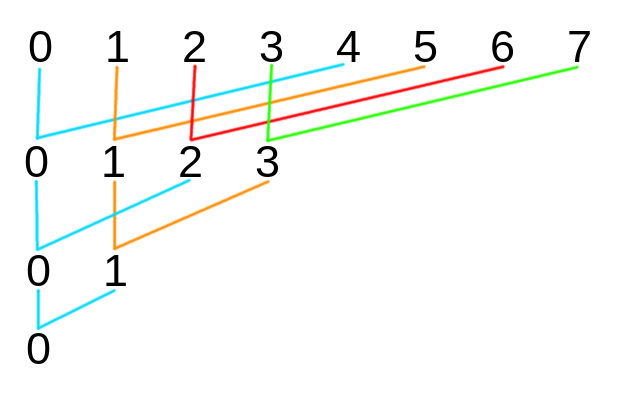
\includegraphics[width=0.5\textwidth]{merge_multi.png}
	\caption{Process Diagram For Mergeing Data Down}
	\label{merge_multi}
\end{figure}

So this is my final plan before I have even written any code for it.
The master who has the list will break it up and send sections to the worker threads using MPI\_Scatter.
When each worker has finished their sorting, they send it to another node using the tree pattern like what MPI\_Reduce might use.
Using this, the sorted list eventually works it's way back up to the master process who will do the final merge of the sorted parts.
You can see the tree reduction in fig\ref{merge_multi} for getting back to the master thread.

\subsection{Time Comparisons}

\begin{figure} [ht]
	\centering
	\begin{tabular}{|l|r|}
		\hline
		& Time  \\ \hline
		MPI (4 threads)&5716330 \\ \hline
		MPI (8 threads)&8120605 \\ \hline
		MPI (2 threads)&10940588\\ \hline
		Reference&17910059      \\ \hline
		\hline
		MPI (4 threads,optimised)&5567745 \\ \hline
		Reference (optimised)&10480717\\ \hline
	\end{tabular}
	\caption{Sorting Time in Microseconds for 100 Million Items}
	\label{sorting_time1}
\end{figure}

So after getting things done, the version using MPI on only my local system is faster!
This is good news that spreading it across 4 cores does help, because I feel vindicated as to my skill of splitting tasks up.
This test for having only 4 threads (one per physical core) on my machine is the fastest which makes sense because it can use every core to it's fullest without stepping on other processes.
I think that it does not scale with more processes because me machine does not have enough hardware for it.
But looking at the optimal multi-process, it does not scale perfectly.
If you multiply the time by 4, it is 22 seconds, where the reference only took 17 seconds.
This shows that there is overhead still in play, but is worth it to split the task up.

One thing that is interesting is when we start trying to pass optimizer flags to the compiler.
Doing the normal level optimizing, the reference code gets a fair bit faster.
But the same flags for the MPI version sees very little improvment.
I have no clue what that means, but with this, the gap is seriously reduced.
With this smaller gap, the benifit is diminished, and so would require even larger projects to justify the extra coding time MPI takes.

I should mention a caveat with my code; it only scales to powers of 2 for processes.
The merging during the sort makes the lowest order processes take data from the higher orders.
While this is great for being a distributed work load for the merge, it does mean that sometimes a stragler process is left out.
If I had more time, I could try implementing an idea I have for leftover process that don't even divide at every step, but for testing, the code would not really be different enough to matter.

\subsection{MPI on Multiple Systems}

So all is well and good for running on the same computer, but if that was all we were going to do, we might as well use a lighter weight multi-threading setup.
Where MPI is very useful is having processes on different systems communicate over a fast interlink.
I took a look online for how to do it and the first link was this
\hyperlink{http://mpitutorial.com/tutorials/running-an-mpi-cluster-within-a-lan/}{source.}

So it seems that you have to have a dedicated list of IPs for every machine you want it to run on.
This seems fine for a static enviroment like a super computer, but I don't think it is capable of dynamicly changing the number of processes.
This means that it is limited to some degree, and requires knowing and managing the resources you need before running.
I could be wrong, but there are too many functions on the reference page for MPI.

\section{Pthreads - The Old Workhorse}

Since the early days of unix, simple APIs for doing things have been a staple.
Pthreads comes from this early time, and with their simple function calls allow programs to do multi-threading.

To use these in this paper, I am (again) going to try making a merge sort.
So my thoughts on how to do this; I have my reference program from the previous section that does all the tricky bits, so I will just modify that.
My first attempt was to intercept where I was splitting the list into smaller pieces recursivly and simply make each split a new thread.
You can see the simple change I made in fig\ref{bad_recursive_threading} where a single line turns into several.

\begin{figure}[htb]
	\centering
	\begin{tabular}{ c }
		\hline
		\begin{minipage}[t]{0.9\textwidth}
		\begin{minted}[frame=none]{c++}
			for(every half of data){
				//recursivly cut down the data
				bool swap_left =
				merge_sort_recurse(buf,half,work);
			}
		\end{minted}
		\end{minipage}
		\\ \hline
		\begin{minipage}[t]{0.9\textwidth}
		\begin{minted}[frame=none]{c++}
			void* merge_sort_recurse_wrapper(void* param_pointer){
				Params* param = (Params*) param_pointer;
				*(param->return_value) = merge_sort_recurse(
						param->buf,param->size,param->work);
				return NULL;
			}
			for(every half of data){
				Params left={&swap_left,buf,half,work}
				pthread_t handle;
				pthread_create(handles,NULL,merge_sort_recurse_wrapper,&left);
				pthread_join(handles[0],NULL);
			}
		\end{minted}
		\end{minipage}
		\\ \hline
	\end{tabular}
	% \vspace{-20pt}
	\caption{Multi-Threaded Recursion ; Top-Original, Bottom-Threaded}
	\label{bad_recursive_threading}
\end{figure}

It works by simply wrapping my original function that recursivly divides the data called "merge\_sort\_recurse".
The original function would split the data in half, check the size, split in half, check the size, until there were only 2 items.
Then it comes back up and does the merging that gives the algorithum it's name.
So the minor change was to have it make a new thread everytime it split the data in half.

This worked just fine when I did my first test on a small list of only 10 elements.
But when I asked it to do real work, it simply segfaults.
The tipping point seems to be going from 10k to 100k items in the list, where there are just too many threads spawned for my computer to handle.
So that means this technique does not scale well enough for my taste and I need to try something else.

So perhaps the way to do it is spawn a set number of worker threads and then throw work at them.
This will not be the same as the MPI system where each thread is given all the data and when they finish they die off.
Instead I am thinking of posting jobs to a global list somehow and each thread will take a job to do on it's own.
The concept is mostly summed up in fig\ref{pthread_psedo} even though it will require a lot more in the way of specifics.

\begin{figure}[htb]
	\centering
	\begin{minipage}[t]{0.9\textwidth}
	\begin{minted}{c++}
		while(num_threads < wanted_number)
			start_worker_thread();
		for(every section of data)
			add_data_section_to_list(section);
	\end{minted}
	\end{minipage}
	\begin{minipage}[t]{0.9\textwidth}
	\begin{minted}{c++}
		void worker_thread(){
			while(have_data_segments){
				data_segment = get_first_item_off_list();
				sort(data_segment);
			}
		}
	\end{minted}
	\end{minipage}
	% \vspace{-20pt}
	\caption{Psudo Code For Pthread}
	\label{pthread_psedo}
\end{figure}

So making a global work queue, what does that look like?
There will be a global variable to point to the object, there will be a mutex to keep things sane.
Seems fairly easy if I just make a linked list with the parameters I need.
You can see a sortend version of it in fig\ref{pthread_psedo_2}.

\begin{figure}[htb]
	\centering
	\begin{minipage}[t]{0.9\textwidth}
	\begin{minted}{c++}
		struct list_item{list_item* next;int *buf,size,*work;};
		pthread_mutex_t queue_mutex;
		struct list_item *list_front=NULL,*list_back=NULL;
		void add_work_item(int*buf,int size,int*work);
		struct list_item* get_next_work(){
			pthread_mutex_lock(&queue_mutex);
			//manage the list
			pthread_mutex_unlock(&queue_mutex);
			return work_item;
		}
	\end{minted}
	\end{minipage}
	% \vspace{-20pt}
	\caption{Psudo Code For Pthread Attempt 2}
	\label{pthread_psedo_2}
\end{figure}

And then for the worker thread, it is fairly simple for shuffling data around.
Ask for work, make sure you actually got some, sort the item or exit. fig\ref{pthread_psedo_3}

\begin{figure}[htb]
	\centering
	\begin{minipage}[t]{0.9\textwidth}
	\begin{minted}{c++}
		void* worker_thread(void*){
			auto segment = get_next_work();
			while(segment != NULL){
				merge_sort_sort(segment);
				segment = get_next_work();
			}
		}
		pthread_t handles[NUM_THREADS];
		for(int x=0; x<NUM_THREADS; x++)
			pthread_create(handles+x,NULL,worker_thread,NULL);
		for(int x=0; x<NUM_THREADS; x++)
			pthread_join(handles[x],NULL);
	\end{minted}
	\end{minipage}
	% \vspace{-20pt}
	\caption{Psudo Code For Pthread Attempt 2 - Worker}
	\label{pthread_psedo_3}
\end{figure}

So with me implementing in code, how does it compare?
The gory numbers are show in fig\ref{sorting_time2}.
The way I am doing the sorting is apparently very terrible, with more threads just making things worse.

\begin{figure} [ht]
	\centering
	\begin{tabular}{|l|r|}
		\hline
		& Time  \\ \hline
		MPI (4 threads)&5716330      \\ \hline
		Pthreads(1 threads)&17771804 \\ \hline
		Reference&17910059           \\ \hline
		Pthreads(2 threads)&29780136 \\ \hline
		Pthreads(4 threads)&32644114 \\ \hline
		Pthreads(8 threads)&36312550 \\ \hline
		\hline
		MPI (4 threads,optimised)&5567745 \\ \hline
		Reference (optimised)&10480717\\ \hline
		Pthread (2 threads,optimised)&26507091 \\ \hline
	\end{tabular}
	\caption{Sorting Time in Microseconds for 100 Million Items}
	\label{sorting_time2}
\end{figure}

I believe that the problem comes from the way I am passing out work.
There is a mutex to lock for every time a thread wants to get more work to do, which is an expensive operation.
I would need to fundamentally change the way my program works if I want to correct this problem.
I likely would try adding a job queue to every thread instead so that there are multiple contention points, and not just a single one.

There is possibly another problem that I don't think is much of the stall time.
Since it must merge groups together, there is a dependency for some jobs to use data from other jobs that should already be calculated.
I did not seperate the jobs out quite right, so there is likely some threads waiting for other to finish first.

But alas, I am out of time to work on this, and we will see if things work out any better in the next section.

\subsection{v2}

So I HAD to make this work in a different manner, which was a fairly large code change.
The difference is that the setup of the threads is no longer recursive.
There are some benifits to my new code.

\begin{itemize}
	\item Can use the source to do the OpenMP section because I now have loops
	\item Slightly faster even though the work queue is almost exactly the same
	\item The sorting now gives back correct results
	\item No weird dependency graph as much as before because things are stacked better this time
	\item Works for ANY number of threads, even prime numbers!
\end{itemize}

\begin{figure} [ht]
	\centering
	\begin{tabular}{|l|r|}
		\hline
		& Time  \\ \hline
		MPI (4 threads)&5716330      \\ \hline
		Reference&17910059           \\ \hline
		Pthreads(1 threads)&21065220 \\ \hline
		Pthreads(4 threads)&21312523 \\ \hline
		Pthreads(2 threads)&23772001 \\ \hline
		Pthreads(8 threads)&23410093 \\ \hline
		\hline
		MPI (4 threads,optimised)&5567745 \\ \hline
		Reference (optimised)&10480717\\ \hline
		Pthread (4 threads,optimised)&17753379 \\ \hline
		Pthread (2 threads,optimised)&20213911 \\ \hline
	\end{tabular}
	\caption{Sorting Time in Microseconds for 100 Million Items}
	\label{sorting_time2a}
\end{figure}

\section{OpenMP}

This is a really neat thing, where the compiler has it built in for implicitly multi-threading things.
Also, by using pragmas to give directives, if a compiler does not understand what you want, then it can safely ignore it and just make you program single-threaded without any changes.
I was so excited about this that I pulled up one of my old projects and tried to make it run faster!

\begin{figure}[ht]
	\centering
	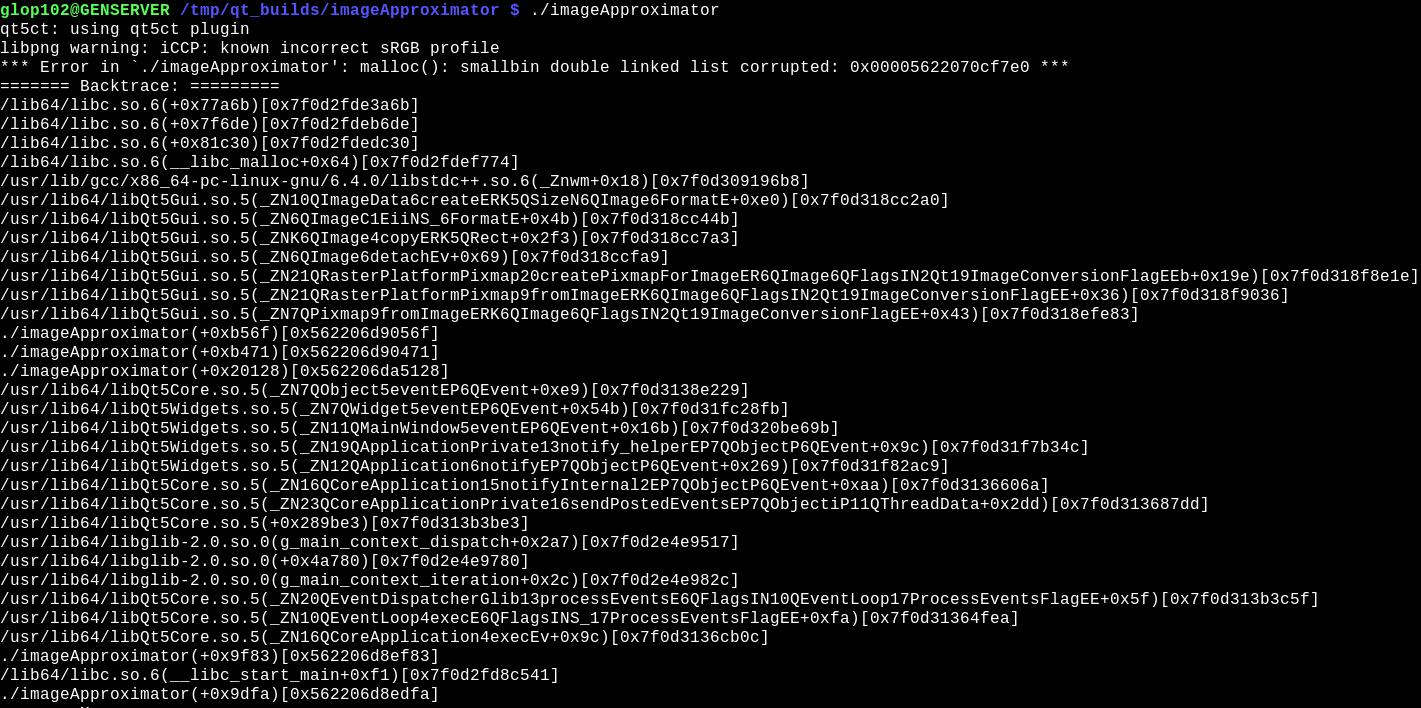
\includegraphics[width=0.6\textwidth]{openMP_for_image_approximator.png}
	\caption{malloc() Corruption Issue Somehow}
	\label{openmp_fail1}
\end{figure}

Well, that is to be expected I guess. It was my first attempt at OpenMP and I had not even skimmed the book yet.
So after that, I did the MPI part of the paper.

So how will I demonstrate my learning about OpenMP?
There previous two sections were variously sucessful modifications of merge sort, so that is where I started this time also.
Being a good lazy programmer, I wanted to try the easiest solution first; where are my for loops?
Besides having a few that did some minor cleanup work, there are none.
This has been my problem with the pthreads, no easy loops to work with because I made everything recursive.

So there are 3 options; make the program use loops instead of recursion, do another topic, give up because the paper is due in a couple hours.
While I seriously considered the last option, there is still time to try the others.
I spun the gears in my head to come up with a new idea to work on, but my creativity does not work that way.
Seems I'm stuck working with what I have.

%went back and made the v2 part of the pthreads section

After having modified the pthreads version to be non-recursive (and other benifits), it should be easier to try out OpenMP.
Like before, I look for any loops that I can directly add OpenMP onto.
Unfortunantly, the only for loops are in the queue init function and have lost of dependencies on previous state.
That means I am stuck with looking only at the threads coming off the work queue.
Luckily it was fairly simple to convert the pthread code to the openmp code.

Fig\ref{openmp_psedo1} shows the comparison of the different codes.
The only major change is how I define the mutex for getting work from the queue.
The mutex used to be burried in the get\_work() function, but now I am specifing the assignment as critical.
The barrier condition is a little funny looking now, but it seems to work.
Starting the various threads is shorter and nicer looking.

\begin{figure}[htb]
	\centering
	\begin{minipage}[t]{0.9\textwidth}
	\begin{minted}{c++}
		void* worker_thread(void*){
			auto segment = get_next_work();
			while(segment != NULL){
				if(segment->left!=NULL)
					merge_sort_merge(segment);
				else // sync command
					pthread_barrier_wait(&sync_barrier);
				segment = get_next_work();
			}
		}
		pthread_t handles[NUM_THREADS];
		for(int x=0; x<NUM_THREADS; x++)
			pthread_create(handles+x,NULL,worker_thread,NULL);
		for(int x=0; x<NUM_THREADS; x++)
			pthread_join(handles[x],NULL);
	\end{minted}
	\end{minipage}
	\begin{minipage}[t]{0.9\textwidth}
	\begin{minted}{c++}
		void* worker_thread(void*){
			#pragma omp critical
			auto segment = get_next_work();
			while(segment != NULL){
				if(segment->left!=NULL)
					merge_sort_merge(segment);
				else{ // sync command
					#pragma omp barrier
					;}
				#pragma omp critical
				segment = get_next_work();
			}
		}
		#pragma omp parallel num_threads(NUM_THREADS)
		worker_thread(NULL);
	\end{minted}
	\end{minipage}
	% \vspace{-20pt}
	\caption{Psudo Code For Pthread Attempt 2 - Worker}
	\label{openmp_psedo1}
\end{figure}

\clearpage
Lets look at the times now in fig\ref{sorting_time3}.
Since the code is almost exactly the pthread code, it makes sense that it is in the same ballpark.
What I find intersting though is how there seems to be less variance in the times between the number of threads.
There was so little variance, that it took 32 threads before there was more than margin of error, and then it went down in time.
(Honestly no clue as to what it is doing)
The optimised times show a less drastic improvment that the pthreads, but there still is some.

\begin{figure} [ht]
	\centering
	\begin{tabular}{|l|r|}
		\hline
		& Time  \\ \hline
		MPI (4 threads)&5716330      \\ \hline
		Reference&17910059           \\ \hline
		OpenMP(32 threads)&19705202 \\ \hline
		OpenMP (8 threads)&20043185 \\ \hline
		OpenMP (2 threads)&20158438 \\ \hline
		OpenMP(16 threads)&20272851 \\ \hline
		OpenMP (4 threads)&20741977 \\ \hline
		OpenMP (1 threads)&20845935 \\ \hline
		Pthreads(4 threads)&21312523 \\ \hline
		\hline
		MPI (4 threads,optimised)&5567745 \\ \hline
		Reference (optimised)&10480717\\ \hline
		OpenMP (2 threads,optimised)&16650686 \\ \hline
		OpenMP (8 threads,optimised)&17425908 \\ \hline
		Pthread (4 threads,optimised)&17753379 \\ \hline
		OpenMP (4 threads,optimised)&18311526 \\ \hline
	\end{tabular}
	\caption{Sorting Time in Microseconds for 100 Million Items}
	\label{sorting_time3}
\end{figure}

\newpage
\clearpage
\appendix
\section{reference.cpp}

\begin{minted}{c++}
#include <stdio.h>
#include <stdlib.h>
#include <time.h>
#include <unistd.h>
#include <sys/time.h>

void merge_sort();

int main(){
	merge_sort();
	return 0;
}


#define LIST_SIZE 100000000
bool merge_sort_recurse(int* buf,int size,int* work);
void merge_sort_merge(int* left_buf,int left_size,int* right_buf,int right_size,int* dest);
void merge_sort(){
	struct timeval timecheck;
	long start_time,end_time;
	srand(time(NULL));

	int* buf = (int*)malloc(LIST_SIZE*sizeof(int));
	int* work = (int*)malloc(LIST_SIZE*sizeof(int));
	for(int i=0;i<LIST_SIZE;i++)
		buf[i] = (rand()/(double)(RAND_MAX)) * LIST_SIZE;

	gettimeofday(&timecheck, NULL);
	start_time = (long)timecheck.tv_sec * 1000000 + (long)timecheck.tv_usec;
	bool is_backwards =
	merge_sort_recurse(buf,LIST_SIZE,work);
	gettimeofday(&timecheck, NULL);
	end_time = (long)timecheck.tv_sec * 1000000 + (long)timecheck.tv_usec;

	// for(int x=0; x<LIST_SIZE; x++)
	// 	if(is_backwards)
	// 		printf("%d  ", work[x]);
	// 	else
	// 		printf("%d  ", buf[x]);
	// printf("\n");
	printf("Time Taken in us : %ld\n",end_time - start_time);
	free(buf);
	free(work);
}
bool merge_sort_recurse(int* buf,int size,int* work){
	if(size==1){
		// *work = *buf;
		return false;
	}
	if(size==2){
		if(buf[0] > buf[1]){
			int temp = buf[1];
			buf[0] = buf[1];
			buf[1] = temp;
		}
		// work[0] = buf[0];
		// work[1] = buf[1];
		//printf("  %d  %d\n\n",work[0],work[1]);
		return false;
	}
	// recursive part
	int half = size/2;
	bool swap_left=false,swap_right=false;
		swap_left =
		merge_sort_recurse(buf,half,work);
		swap_right =
		merge_sort_recurse(buf+half,size-half,work+half); // subtraction for odd sizes
	if(swap_left != swap_right){
		if(swap_right)
			for(int i=0; i<half; i++)
				work[i] = buf[i];
		else
			for(int i=0; i<half; i++)
				buf[i] = work[i];
			
	}
	if(swap_right){
		int* temp = work;
		work = buf;
		buf = temp;
	}
	merge_sort_merge(buf,half,buf+half,size-half,work);

	return !swap_right;
}
void merge_sort_merge(int* left_buf,int left_size,int* right_buf,int right_size,int* dest){
	while(left_size && right_size){
		if(*left_buf <= *right_buf){
			*dest = *left_buf;
			left_size--;
			left_buf++;
		}else{
			*dest = *right_buf;
			right_size--;
			right_buf++;
		}
		dest++;
	}
	while(left_size){
		*dest = *left_buf;
		left_size--;
		left_buf++;
		dest++;
	}
	while(right_size){
		*dest = *right_buf;
		right_size--;
		right_buf++;
		dest++;
	}

	return;
}
\end{minted}

\newpage
\clearpage
\section{mpi.cpp}
\begin{minted}{c++}
#include <stdio.h>
#include <string.h>
#include <mpi.h>
#include <sys/time.h>

void hello_world_wikipedia();
void hello_world_book();
void hello_world_masterOnlySend();
void merge_sort();

int main(int argc, char **argv)
{
	//hello_world_wikipedia();
	//hello_world_book();
	//hello_world_masterOnlySend();
	merge_sort();
	return 0;
}

void hello_world_wikipedia(){
	char buf[256];
	int my_rank, num_procs;

	/* Initialize the infrastructure necessary for communication */
	MPI_Init(NULL,NULL);
	MPI_Comm_rank(MPI_COMM_WORLD, &my_rank);
	MPI_Comm_size(MPI_COMM_WORLD, &num_procs);

	if (my_rank == 0) {
		int other_rank;
		printf("We have %i processes.\n", num_procs);

		/* Send messages to all other processes */
		for (other_rank = 1; other_rank < num_procs; other_rank++){
			sprintf(buf, "Hello %i!", other_rank);
			MPI_Send(buf, sizeof(buf), MPI_CHAR, other_rank, 0, MPI_COMM_WORLD);
		}

		/* Receive messages from all other process */
		for (other_rank = 1; other_rank < num_procs; other_rank++){
			MPI_Recv(buf, sizeof(buf), MPI_CHAR, other_rank, 0, MPI_COMM_WORLD, MPI_STATUS_IGNORE);
			printf("%s\n", buf);
		}

	}else{

		/* Receive message from process #0 */
		MPI_Recv(buf, sizeof(buf), MPI_CHAR, 0, 0, MPI_COMM_WORLD, MPI_STATUS_IGNORE);

		/* Send message to process #0 */
		sprintf(buf, "Process %i reporting for duty.", my_rank);
		MPI_Send(buf, sizeof(buf), MPI_CHAR, 0, 0, MPI_COMM_WORLD);

	}

	/* Tear down the communication infrastructure */
	MPI_Finalize();
}

void hello_world_masterOnlySend(){
	char buf[256];
	int my_rank, num_procs;

	/* Initialize the infrastructure necessary for communication */
	MPI_Init(NULL,NULL);
	MPI_Comm_rank(MPI_COMM_WORLD, &my_rank);
	MPI_Comm_size(MPI_COMM_WORLD, &num_procs);

	if (my_rank == 0) {
		printf("Master process of %d processes\n",num_procs);

		for (int other_rank = 1; other_rank < num_procs; other_rank++){
			sprintf(buf,"Process %d of %d",other_rank,num_procs);
			MPI_Send(buf, strlen(buf)+1, MPI_CHAR, other_rank, 0, MPI_COMM_WORLD);
		}
	}else{
		MPI_Recv(buf, sizeof(buf), MPI_CHAR, 0, 0, MPI_COMM_WORLD, MPI_STATUS_IGNORE);
		printf("%s\n",buf);
	}

	/* Tear down the communication infrastructure */
	MPI_Finalize();
}

void hello_world_book(){
	char buf[256];
	int my_rank, num_procs;

	/* Initialize the infrastructure necessary for communication */
	MPI_Init(NULL,NULL);
	MPI_Comm_rank(MPI_COMM_WORLD, &my_rank);
	MPI_Comm_size(MPI_COMM_WORLD, &num_procs);

	if (my_rank == 0) {
		printf("Master process of %d processes\n",num_procs);

		for (int other_rank = 1; other_rank < num_procs; other_rank++){
			MPI_Recv(buf, sizeof(buf), MPI_CHAR, other_rank, 0, MPI_COMM_WORLD,MPI_STATUS_IGNORE);
			printf("%s\n",buf);
		}
	}else{
		sprintf(buf,"Process %d of %d",my_rank,num_procs);
		MPI_Send(buf, strlen(buf)+1, MPI_CHAR, 0, 0, MPI_COMM_WORLD);
	}

	/* Tear down the communication infrastructure */
	MPI_Finalize();
}


#define LIST_SIZE 100000000
bool merge_sort_recurse(int* buf,int size,int* work);
void merge_sort_merge(int* left_buf,int left_size,int* right_buf,int right_size,int* dest);
bool gather_tree(int* local_buf,int* local_work,int local_buf_len,int num_procs,int my_rank);
void merge_sort(){
	struct timeval timecheck;
	long start_time,end_time;
	int my_rank, num_procs;
	srand(time(NULL));

	MPI_Init(NULL,NULL);
	MPI_Comm_rank(MPI_COMM_WORLD, &my_rank);
	MPI_Comm_size(MPI_COMM_WORLD, &num_procs);

	int local_buf_len = LIST_SIZE / num_procs; // how elements are in normal buffs
	int buf_extra_elms = LIST_SIZE - local_buf_len*num_procs; // how many extra elms the master will have to do itself
	int* local_buf = (int*)malloc(LIST_SIZE*sizeof(int));
	int* local_work = (int*)malloc(LIST_SIZE*sizeof(int));

	if(my_rank == 0){
		int* buf = (int*)malloc(LIST_SIZE*sizeof(int));
		for(int i=0;i<LIST_SIZE;i++)
			buf[i] = (rand()/(double)(RAND_MAX)) * LIST_SIZE;

		MPI_Barrier(MPI_COMM_WORLD);
		gettimeofday(&timecheck, NULL);
		start_time = (long)timecheck.tv_sec * 1000000 + (long)timecheck.tv_usec;

		MPI_Scatter(buf, local_buf_len, MPI_INT,
			local_buf, local_buf_len, MPI_INT, 0,
			MPI_COMM_WORLD);
		for(int x=0; x<buf_extra_elms; x++)
			local_buf[x+local_buf_len] = buf[x + (local_buf_len*num_procs)];
		bool swapped =
		merge_sort_recurse(local_buf,local_buf_len+buf_extra_elms,local_work);

		int extras[buf_extra_elms];
		for(int x=0; x<buf_extra_elms; x++)
			extras[x] = local_buf[x+local_buf_len];

		if(swapped){
			int* temp = local_buf;
			local_buf = local_work;
			local_work = temp;
		}
		swapped = gather_tree(local_buf,local_work,local_buf_len,num_procs,my_rank);
		free(buf);
	}else{
		MPI_Barrier(MPI_COMM_WORLD);
		MPI_Scatter(NULL, 0, MPI_INT,
			local_buf, local_buf_len, MPI_INT, 0,
			MPI_COMM_WORLD);
		bool swapped =
		merge_sort_recurse(local_buf,local_buf_len,local_work);

		if(swapped){
			int* temp = local_buf;
			local_buf = local_work;
			local_work = temp;
		}
		swapped = gather_tree(local_buf,local_work,local_buf_len,num_procs,my_rank);
	}

	MPI_Barrier(MPI_COMM_WORLD);

	if(my_rank == 0){
		gettimeofday(&timecheck, NULL);
		end_time = (long)timecheck.tv_sec * 1000000 + (long)timecheck.tv_usec;

		printf("Time Taken : %ld\n",end_time - start_time);
	}

	free(local_buf);
	free(local_work);

	MPI_Finalize();
}
bool merge_sort_recurse(int* buf,int size,int* work){
	if(size==1){
		// *work = *buf;
		return false;
	}
	if(size==2){
		if(buf[0] > buf[1]){
			int temp = buf[1];
			buf[0] = buf[1];
			buf[1] = temp;
		}
		// work[0] = buf[0];
		// work[1] = buf[1];
		//printf("  %d  %d\n\n",work[0],work[1]);
		return false;
	}
	// recursive part
	int half = size/2;
	bool swap_left=false,swap_right=false;
		swap_left =
		merge_sort_recurse(buf,half,work);
		swap_right =
		merge_sort_recurse(buf+half,size-half,work+half); // subtraction for odd sizes
	if(swap_left != swap_right){
		if(swap_right)
			for(int i=0; i<half; i++)
				work[i] = buf[i];
		else
			for(int i=0; i<half; i++)
				buf[i] = work[i];
			
	}
	if(swap_right){
		int* temp = work;
		work = buf;
		buf = temp;
	}
	merge_sort_merge(buf,half,buf+half,size-half,work);

	return !swap_right;
}

void merge_sort_merge(int* left_buf,int left_size,int* right_buf,int right_size,int* dest){
	while(left_size && right_size){
		if(*left_buf <= *right_buf){
			*dest = *left_buf;
			left_size--;
			left_buf++;
		}else{
			*dest = *right_buf;
			right_size--;
			right_buf++;
		}
		dest++;
	}
	while(left_size){
		*dest = *left_buf;
		left_size--;
		left_buf++;
		dest++;
	}
	while(right_size){
		*dest = *right_buf;
		right_size--;
		right_buf++;
		dest++;
	}

	return;
}

//0 1 2 3 4 5 6 7 8 9
//0 1 2 3 4
//0 1 2
//0    2

//0 1 2 3 4 5 6 7 8
//0 1 2 3          8
//0 1              8
//0                8

//0 1 2 3 4 5 6 7
//0 1 2 3
//0 1
//0

//0 1 2 3 4 5 6     h=3
//0 1 2        6    h=1
//0 1  2       6    h=1
//0    2       6    h=0
bool gather_tree(int* local_buf,int* local_work,int local_buf_len,int num_procs,int my_rank){
	bool swapped = false;

	int half = num_procs/2;
	int extra_proc=0,extra_size;
	while(half){
		if(my_rank<half){
			MPI_Recv(local_buf+local_buf_len, local_buf_len, MPI_INT, my_rank+half, 0, MPI_COMM_WORLD,MPI_STATUS_IGNORE);
			merge_sort_merge(local_buf,local_buf_len,local_buf+local_buf_len,local_buf_len,local_work);
		}else if(my_rank<(2*half)){
			MPI_Send(local_buf, local_buf_len, MPI_INT, my_rank-half, 0, MPI_COMM_WORLD);
			return swapped; //we gave our work to someone else, so we are done
		}else{
			// printf("%d is extra\n",my_rank);
			// if(extra_proc==0){
			// 	extra_proc = my_rank;
			// 	extra_size = local_buf_len;
			// }else{
			// 	if(extra_proc == my_rank){
			// 		MPI_Send(local_buf, extra_size, MPI_INT, my_rank-half, 0, MPI_COMM_WORLD);
			// 		return swapped; //we gave our work to someone else, so we are done
			// 	}else{
			// 		MPI_Recv(local_buf+local_buf_len, local_buf_len, MPI_INT, my_rank+half, 0, MPI_COMM_WORLD,MPI_STATUS_IGNORE);
			// 		merge_sort_merge(local_buf,local_buf_len,local_buf+local_buf_len,local_buf_len,local_work);
			// 	}
			// 	extra_proc = 0;
			// }
		}
		half/=2;
		local_buf_len*=2;
		swapped = !swapped;
		int* temp = local_buf;
		local_work = local_buf;
		local_buf=temp;
	}
	return swapped;
}
\end{minted}


\newpage
\clearpage
\section{pthread2.cpp}
\begin{minted}{c++}
#include <stdio.h>
#include <stdlib.h>
#include <time.h>
#include <unistd.h>
#include <sys/time.h>
#include <pthread.h>

#define LIST_SIZE 100000000
// #define LIST_SIZE 10
#define NUM_THREADS 2

void merge_sort();

int main(){
	merge_sort();
	return 0;
}

struct list_item{list_item* next;int *left,*right,left_size,right_size,*work;};
pthread_mutex_t queue_mutex;
pthread_barrier_t sync_barrier;
struct list_item *list_front=NULL,*list_back=NULL;
void add_work_item(int*left,int*right,int left_size,int right_size,int*work){
	//printf("%d  %d\n",left_size,right_size);
	//pthread_mutex_lock(&queue_mutex);
	struct list_item *prev = list_back;
	list_back = new struct list_item;
	list_back->next=NULL;
	list_back->left=left;
	list_back->left_size=left_size;
	list_back->right=right;
	list_back->right_size=right_size;
	list_back->work=work;
	if(list_front == NULL){
		list_front = list_back;
	}
	if(prev != NULL)
		prev->next = list_back;
	//pthread_mutex_unlock(&queue_mutex);
}
struct list_item* get_next_work(){
	pthread_mutex_lock(&queue_mutex);
	struct list_item* temp = list_front;
	if(temp != NULL)
		list_front = list_front->next;
	pthread_mutex_unlock(&queue_mutex);
	return temp;
}
// bool init_work_list(int*buf,int size,int*work){
// 	if(size<=2){
// 		add_work_item(buf,size,work);
// 		return false;
// 	}
// 	int half = size/2;
// 	bool swap_left = init_work_list(buf,half,work);
// 	bool swap_right = init_work_list(buf+half,size-half,work+half);
// 	if(swap_left != swap_right){
// 		if(swap_right)
// 			for(int i=0; i<half; i++)
// 				work[i] = buf[i];
// 		else
// 			for(int i=0; i<half; i++)
// 				buf[i] = work[i];
			
// 	}
// 	if(swap_right){
// 		int* temp = work;
// 		work = buf;
// 		buf = temp;
// 	}

// 	add_work_item(buf,half,work);
// 	add_work_item(buf+half,size-half,work+half);
// 	//add_work_item(NULL,0,NULL);

// 	return !swap_right;
// }

bool init_work_2(int*buf,int size,int*work){
	bool swapped = false;
	int step=2;
	//handle the base cases first
	for(int x=0; x<size; x+=2){
		if(x+2<=size){
			add_work_item(buf+x,NULL,2,0,work+x);
		}else
			add_work_item(buf+x,NULL,1,0,work+x);
	}
	// sync all the threads
	for(int x=0; x<NUM_THREADS; x++)
		add_work_item(NULL,NULL,0,0,NULL);

	//now the merging part
	while(step<size){
		for(int curt_step=0; curt_step<size; curt_step+=2*step){
			if(curt_step+2*step<size){
				//normal full merge
				add_work_item(buf+curt_step,buf+curt_step+step,step,step,work+curt_step);
			}else if(curt_step+step<size){
				//left full size, right partial size
				int partial = size - (curt_step+step);
				add_work_item(buf+curt_step,buf+curt_step+step,step,partial,work+curt_step);
			}else{
				//left partial size
				int partial = size - curt_step;
				add_work_item(buf+curt_step,NULL,partial,0,work+curt_step);
			}
		}
		// sync all the threads
		for(int x=0; x<NUM_THREADS; x++)
			add_work_item(NULL,NULL,0,0,NULL);
		
		step*=2;
		swapped = !swapped;
		int*temp = buf;
		buf=work;
		work=temp;
	}
	return swapped;
}


void* worker_thread(void*);
void merge_sort_sort(int* buf,int size,int* work);
void merge_sort_merge(int* left_buf,int left_size,int* right_buf,int right_size,int* dest);
void merge_sort(){
	struct timeval timecheck;
	long start_time,end_time;
	srand(time(NULL));
	pthread_mutex_init(&queue_mutex,NULL);
	pthread_barrier_init(&sync_barrier,NULL,NUM_THREADS);

	int* buf = (int*)malloc(LIST_SIZE*sizeof(int));
	int* work = (int*)malloc(LIST_SIZE*sizeof(int));
	for(int i=0;i<LIST_SIZE;i++)
		buf[i] = (rand()/(double)(RAND_MAX)) * LIST_SIZE;

	gettimeofday(&timecheck, NULL);
	start_time = (long)timecheck.tv_sec * 1000000 + (long)timecheck.tv_usec;
	bool is_backwards =
	//init_work_list(buf,LIST_SIZE,work);
	init_work_2(buf,LIST_SIZE,work);
	{
		pthread_t handles[NUM_THREADS];
		for(int x=0; x<NUM_THREADS; x++)
			pthread_create(handles+x,NULL,worker_thread,NULL);
		for(int x=0; x<NUM_THREADS; x++)
			pthread_join(handles[x],NULL);
	}
	//merge_sort_recurse(buf,LIST_SIZE,work);
	gettimeofday(&timecheck, NULL);
	end_time = (long)timecheck.tv_sec * 1000000 + (long)timecheck.tv_usec;

	// for(int x=0; x<LIST_SIZE; x++)
	// 	if(is_backwards)
	// 		printf("%d  ", work[x]);
	// 	else
	// 		printf("%d  ", buf[x]);
	// printf("\n");
	printf("Time Taken in us : %ld\n",end_time - start_time);
	free(buf);
	free(work);
}
// void merge_sort_sort(int*left,int*right,int size,int* work){
// 	if(size==1){
// 		return;
// 	}
// 	if(size==2){
// 		if(buf[0] > buf[1]){
// 			int temp = buf[1];
// 			buf[0] = buf[1];
// 			buf[1] = temp;
// 		}
// 		return;
// 	}
// 	int half = size/2;
// 	merge_sort_merge(buf,half,buf+half,size-half,work);
// }
void merge_sort_merge(int* left_buf,int left_size,int* right_buf,int right_size,int* dest){
	if(left_size==1 && right_buf == NULL){
		// *dest = *left_buf;
		return;
	}
	if(left_size==2 && right_buf == NULL){
		if(left_buf[0] > left_buf[1]){
			int temp = left_buf[1];
			left_buf[0] = left_buf[1];
			left_buf[1] = temp;
		}
		// dest[0]=left_buf[0];
		// dest[1]=left_buf[1];
		return;
	}
	while(left_size && right_size){
		if(*left_buf <= *right_buf){
			*dest = *left_buf;
			left_size--;
			left_buf++;
		}else{
			*dest = *right_buf;
			right_size--;
			right_buf++;
		}
		dest++;
	}
	while(left_size){
		*dest = *left_buf;
		left_size--;
		left_buf++;
		dest++;
	}
	while(right_size){
		*dest = *right_buf;
		right_size--;
		right_buf++;
		dest++;
	}

	return;
}

void* worker_thread(void*){
	auto segment = get_next_work();
	while(segment != NULL){
		if(segment->left!=NULL)
			merge_sort_merge(segment->left,segment->left_size,segment->right,segment->right_size,segment->work);
		else // sync command
			pthread_barrier_wait(&sync_barrier);
		segment = get_next_work();
	}
}
\end{minted}


\newpage
\clearpage
\section{openmp.cpp}
\begin{minted}{c++}
#include <stdio.h>
#include <stdlib.h>
#include <time.h>
#include <unistd.h>
#include <sys/time.h>
#include <omp.h>

#define LIST_SIZE 100000000
// #define LIST_SIZE 10
#define NUM_THREADS 8

void merge_sort();

int main(){
	merge_sort();
	return 0;
}

struct list_item{list_item* next;int *left,*right,left_size,right_size,*work;};
struct list_item *list_front=NULL,*list_back=NULL;
void add_work_item(int*left,int*right,int left_size,int right_size,int*work){
	//printf("%d  %d\n",left_size,right_size);
	//pthread_mutex_lock(&queue_mutex);
	struct list_item *prev = list_back;
	list_back = new struct list_item;
	list_back->next=NULL;
	list_back->left=left;
	list_back->left_size=left_size;
	list_back->right=right;
	list_back->right_size=right_size;
	list_back->work=work;
	if(list_front == NULL){
		list_front = list_back;
	}
	if(prev != NULL)
		prev->next = list_back;
	//pthread_mutex_unlock(&queue_mutex);
}
struct list_item* get_next_work(){
	struct list_item* temp = list_front;
	if(temp != NULL)
		list_front = list_front->next;
	return temp;
}
// bool init_work_list(int*buf,int size,int*work){
// 	if(size<=2){
// 		add_work_item(buf,size,work);
// 		return false;
// 	}
// 	int half = size/2;
// 	bool swap_left = init_work_list(buf,half,work);
// 	bool swap_right = init_work_list(buf+half,size-half,work+half);
// 	if(swap_left != swap_right){
// 		if(swap_right)
// 			for(int i=0; i<half; i++)
// 				work[i] = buf[i];
// 		else
// 			for(int i=0; i<half; i++)
// 				buf[i] = work[i];
			
// 	}
// 	if(swap_right){
// 		int* temp = work;
// 		work = buf;
// 		buf = temp;
// 	}

// 	add_work_item(buf,half,work);
// 	add_work_item(buf+half,size-half,work+half);
// 	//add_work_item(NULL,0,NULL);

// 	return !swap_right;
// }

bool init_work_2(int*buf,int size,int*work){
	bool swapped = false;
	int step=2;
	//handle the base cases first
	for(int x=0; x<size; x+=2){
		if(x+2<=size){
			add_work_item(buf+x,NULL,2,0,work+x);
		}else
			add_work_item(buf+x,NULL,1,0,work+x);
	}
	// sync all the threads
	for(int x=0; x<NUM_THREADS; x++)
		add_work_item(NULL,NULL,0,0,NULL);

	//now the merging part
	while(step<size){
		for(int curt_step=0; curt_step<size; curt_step+=2*step){
			if(curt_step+2*step<size){
				//normal full merge
				add_work_item(buf+curt_step,buf+curt_step+step,step,step,work+curt_step);
			}else if(curt_step+step<size){
				//left full size, right partial size
				int partial = size - (curt_step+step);
				add_work_item(buf+curt_step,buf+curt_step+step,step,partial,work+curt_step);
			}else{
				//left partial size
				int partial = size - curt_step;
				add_work_item(buf+curt_step,NULL,partial,0,work+curt_step);
			}
		}
		// sync all the threads
		for(int x=0; x<NUM_THREADS; x++)
			add_work_item(NULL,NULL,0,0,NULL);
		
		step*=2;
		swapped = !swapped;
		int*temp = buf;
		buf=work;
		work=temp;
	}
	return swapped;
}


void* worker_thread(void*);
void merge_sort_sort(int* buf,int size,int* work);
void merge_sort_merge(int* left_buf,int left_size,int* right_buf,int right_size,int* dest);
void merge_sort(){
	struct timeval timecheck;
	long start_time,end_time;
	srand(time(NULL));

	int* buf = (int*)malloc(LIST_SIZE*sizeof(int));
	int* work = (int*)malloc(LIST_SIZE*sizeof(int));
	for(int i=0;i<LIST_SIZE;i++)
		buf[i] = (rand()/(double)(RAND_MAX)) * LIST_SIZE;

	gettimeofday(&timecheck, NULL);
	start_time = (long)timecheck.tv_sec * 1000000 + (long)timecheck.tv_usec;
	bool is_backwards =
	//init_work_list(buf,LIST_SIZE,work);
	init_work_2(buf,LIST_SIZE,work);
	#pragma omp parallel num_threads(NUM_THREADS)
	worker_thread(NULL);
	//merge_sort_recurse(buf,LIST_SIZE,work);
	gettimeofday(&timecheck, NULL);
	end_time = (long)timecheck.tv_sec * 1000000 + (long)timecheck.tv_usec;

	// for(int x=0; x<LIST_SIZE; x++)
	// 	if(is_backwards)
	// 		printf("%d  ", work[x]);
	// 	else
	// 		printf("%d  ", buf[x]);
	// printf("\n");
	printf("Time Taken in us : %ld\n",end_time - start_time);
	free(buf);
	free(work);
}
// void merge_sort_sort(int*left,int*right,int size,int* work){
// 	if(size==1){
// 		return;
// 	}
// 	if(size==2){
// 		if(buf[0] > buf[1]){
// 			int temp = buf[1];
// 			buf[0] = buf[1];
// 			buf[1] = temp;
// 		}
// 		return;
// 	}
// 	int half = size/2;
// 	merge_sort_merge(buf,half,buf+half,size-half,work);
// }
void merge_sort_merge(int* left_buf,int left_size,int* right_buf,int right_size,int* dest){
	if(left_size==1 && right_buf == NULL){
		// *dest = *left_buf;
		return;
	}
	if(left_size==2 && right_buf == NULL){
		if(left_buf[0] > left_buf[1]){
			int temp = left_buf[1];
			left_buf[0] = left_buf[1];
			left_buf[1] = temp;
		}
		// dest[0]=left_buf[0];
		// dest[1]=left_buf[1];
		return;
	}
	while(left_size && right_size){
		if(*left_buf <= *right_buf){
			*dest = *left_buf;
			left_size--;
			left_buf++;
		}else{
			*dest = *right_buf;
			right_size--;
			right_buf++;
		}
		dest++;
	}
	while(left_size){
		*dest = *left_buf;
		left_size--;
		left_buf++;
		dest++;
	}
	while(right_size){
		*dest = *right_buf;
		right_size--;
		right_buf++;
		dest++;
	}

	return;
}

void* worker_thread(void*){
	struct list_item* segment;
	#pragma omp critical
	segment = get_next_work();
	while(segment != NULL){
		if(segment->left!=NULL)
			merge_sort_merge(segment->left,segment->left_size,segment->right,segment->right_size,segment->work);
		else{ // sync command
			#pragma omp barrier
			;}
			;
		#pragma omp critical
		segment = get_next_work();
	}
}
\end{minted}


\end{document}
